

\tikzset{every picture/.style={line width=0.3pt}} %set default line width to 0.75pt        

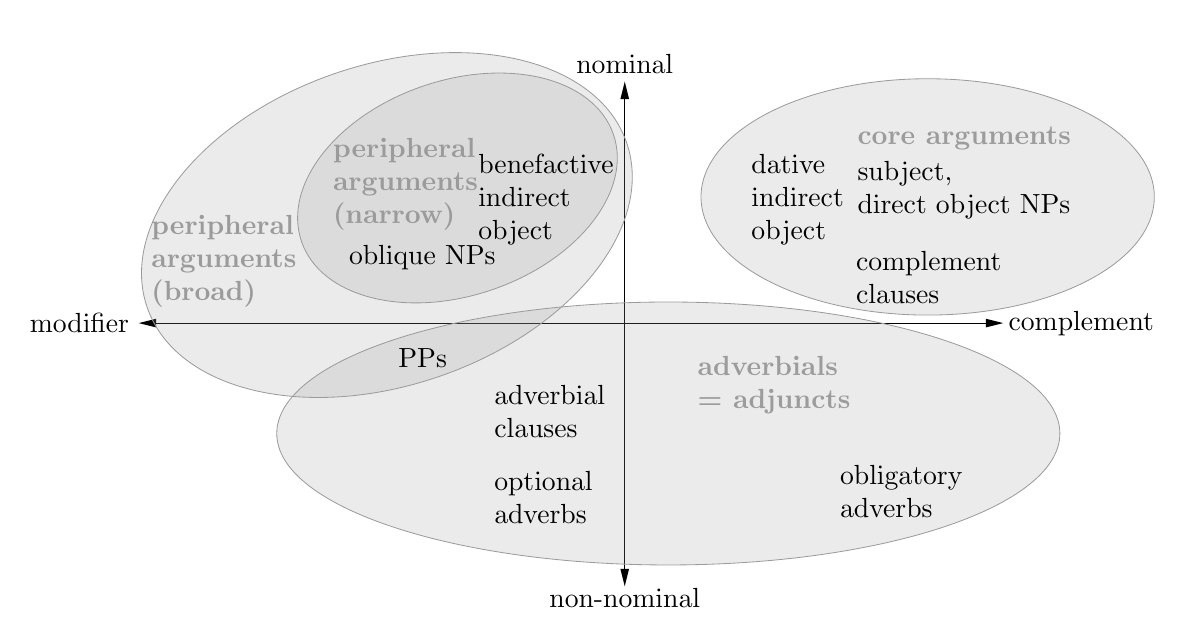
\begin{tikzpicture}[x=0.75pt,y=0.75pt,yscale=-0.7,xscale=0.7]
%uncomment if require: \path (0,401); %set diagram left start at 0, and has height of 401

%Straight Lines [id:da009476237276789146] 
\draw    (80,198) -- (671,198) ;
\draw [shift={(673,198)}, rotate = 180] [fill={rgb, 255:red, 0; green, 0; blue, 0 }  ][line width=0.08]  [draw opacity=0] (12,-3) -- (0,0) -- (12,3) -- cycle    ;
\draw [shift={(78,198)}, rotate = 0] [fill={rgb, 255:red, 0; green, 0; blue, 0 }  ][line width=0.08]  [draw opacity=0] (12,-3) -- (0,0) -- (12,3) -- cycle    ;
%Straight Lines [id:da7773022804601077] 
\draw    (412.5,377.14) -- (412.5,33.86) ;
\draw [shift={(412.5,31.86)}, rotate = 90] [fill={rgb, 255:red, 0; green, 0; blue, 0 }  ][line width=0.08]  [draw opacity=0] (12,-3) -- (0,0) -- (12,3) -- cycle    ;
\draw [shift={(412.5,379.14)}, rotate = 270] [fill={rgb, 255:red, 0; green, 0; blue, 0 }  ][line width=0.08]  [draw opacity=0] (12,-3) -- (0,0) -- (12,3) -- cycle    ;
%Shape: Ellipse [id:dp6612766652403343] 
\draw  [color={rgb, 255:red, 155; green, 155; blue, 155 }  ,draw opacity=1 ][fill={rgb, 255:red, 155; green, 155; blue, 155 }  ,fill opacity=0.2 ] (465,111.15) .. controls (465,66.23) and (534.84,29.81) .. (621,29.81) .. controls (707.16,29.81) and (777,66.23) .. (777,111.15) .. controls (777,156.06) and (707.16,192.48) .. (621,192.48) .. controls (534.84,192.48) and (465,156.06) .. (465,111.15) -- cycle ;
%Shape: Ellipse [id:dp35746311023681887] 
\draw  [color={rgb, 255:red, 155; green, 155; blue, 155 }  ,draw opacity=1 ][fill={rgb, 255:red, 155; green, 155; blue, 155 }  ,fill opacity=0.2 ] (190.01,141.81) .. controls (176.75,103.15) and (214.07,55.33) .. (273.36,34.99) .. controls (332.65,14.66) and (391.46,29.51) .. (404.72,68.17) .. controls (417.98,106.83) and (380.66,154.65) .. (321.37,174.99) .. controls (262.08,195.32) and (203.26,180.47) .. (190.01,141.81) -- cycle ;
%Shape: Ellipse [id:dp7325522804450764] 
\draw  [color={rgb, 255:red, 155; green, 155; blue, 155 }  ,draw opacity=1 ][fill={rgb, 255:red, 155; green, 155; blue, 155 }  ,fill opacity=0.2 ] (83.77,187.11) .. controls (64.01,129.51) and (121.89,57.47) .. (213.03,26.21) .. controls (304.17,-5.05) and (394.07,16.31) .. (413.83,73.91) .. controls (433.58,131.51) and (375.71,203.54) .. (284.57,234.8) .. controls (193.42,266.06) and (103.52,244.71) .. (83.77,187.11) -- cycle ;
%Shape: Ellipse [id:dp17093026002033596] 
\draw  [color={rgb, 255:red, 155; green, 155; blue, 155 }  ,draw opacity=1 ][fill={rgb, 255:red, 155; green, 155; blue, 155 }  ,fill opacity=0.2 ] (173,273.98) .. controls (173,224) and (293.66,183.48) .. (442.5,183.48) .. controls (591.34,183.48) and (712,224) .. (712,273.98) .. controls (712,323.96) and (591.34,364.48) .. (442.5,364.48) .. controls (293.66,364.48) and (173,323.96) .. (173,273.98) -- cycle ;

% Text Node
\draw (571,85) node [anchor=north west][inner sep=0.75pt]   [align=left] {subject,\\ direct object NPs};
% Text Node
\draw (675,198) node [anchor=west] [inner sep=0.75pt]   [align=left] {complement};
% Text Node
\draw (73,198) node [anchor=east] [inner sep=0.75pt]   [align=left] {modifier};
% Text Node
\draw (412.5,27.86) node [anchor=south] [inner sep=0.75pt]   [align=left] {nominal};
% Text Node
\draw (412.5,379.14) node [anchor=north] [inner sep=0.75pt]   [align=left] {non-nominal};
% Text Node
\draw (498,80) node [anchor=north west][inner sep=0.75pt]   [align=left] {dative \\indirect \\object};
% Text Node
\draw (570,147) node [anchor=north west][inner sep=0.75pt]   [align=left] {complement \\clauses};
% Text Node
\draw (310,80) node [anchor=north west][inner sep=0.75pt]   [align=left] {benefactive \\indirect \\object};
% Text Node
\draw (221,143) node [anchor=north west][inner sep=0.75pt]   [align=left] {oblique NPs};
% Text Node
\draw (255,214) node [anchor=north west][inner sep=0.75pt]   [align=left] {PPs};
% Text Node
\draw (559,294) node [anchor=north west][inner sep=0.75pt]   [align=left] {obligatory\\adverbs};
% Text Node
\draw (321,298) node [anchor=north west][inner sep=0.75pt]   [align=left] {optional\\adverbs};
% Text Node
\draw (321,239) node [anchor=north west][inner sep=0.75pt]   [align=left] {adverbial \\clauses};
% Text Node
\draw (571,61) node [anchor=north west][inner sep=0.75pt]  [color={rgb, 255:red, 155; green, 155; blue, 155 }  ,opacity=1 ] [align=left] {\textbf{\textcolor[rgb]{0.61,0.61,0.61}{core arguments}}};
% Text Node
\draw (210,69) node [anchor=north west][inner sep=0.75pt]  [color={rgb, 255:red, 155; green, 155; blue, 155 }  ,opacity=1 ] [align=left] {\textbf{peripheral}\\\textbf{arguments}\\\textbf{(narrow)}};
% Text Node
\draw (85,122) node [anchor=north west][inner sep=0.75pt]  [color={rgb, 255:red, 155; green, 155; blue, 155 }  ,opacity=1 ] [align=left] {\textbf{peripheral }\\\textbf{arguments}\\\textbf{(broad)}};
% Text Node
\draw (461,219) node [anchor=north west][inner sep=0.75pt]   [align=left] {\textcolor[rgb]{0.61,0.61,0.61}{\textbf{adverbials}}\\\textbf{\textcolor[rgb]{0.61,0.61,0.61}{= adjuncts}}};


\end{tikzpicture}
